\apendice{Documentación técnica de programación}

\section{Introducción}

En este anexo se explicarán todos aquellos aspectos relevantes para programadores, desde su estructura de directorios hasta las dependencias que tiene y que haya que instalar en ciertos casos, o el uso de los diferentes archivos que se encuentran en el repositorio.

\section{Estructura de directorios}

Los archivos del proyecto se distribuyen de la siguiente manera:

\begin{itemize}
    \item \verb|/| : contiene ficheros relativos a GitHub, como el ReadMe o la licencia.
    \item \verb|/Material de Tutoriales| : contiene aquellos archivos de código relacionados con los tutoriales y cursos realizados a lo largo del transcurso del proyecto.
    \item \verb|/memoria| : contiene los archivos \LaTeX y PDF de la memoria.
    \item \verb|/code| : carpeta en la que se encuentran todas aquellas subcarpetas que contienen el código del proyecto.
    \item \verb|/code/plainCode| : contiene todas las versiones por las que ha pasado el proyecto, para ejecutarse directamente en la consola sin necesidad de pasar por la página web, ofreciendo un mayor grado de libertad.
    \item \verb|/code/plainCode/tests| : contiene todos los tests unitarios correspondientes a cada una de las versiones del proyecto.
    \item \verb|/code/estudio| : contiene aquellos ficheros relacionados con el estudio de valores óptimos realizado durante el desarrollo del proyecto.
    \item \verb|/code/estudio/resultados_estudio_1| : en esta carpeta se fueron guardando las gráficas obtenidas al realizar el estudio mencionado anteriormente.
    \item \verb|/code/website| : esta carpeta contendrá todos los elementos relacionados con la página web, incluyendo un archivo Dockerfile utilizado a la hora de crear imágenes Docker, y scripts shell para crear una imagen y ejecutarla.
    \item \verb|/code/website/websiteCode| : en esta carpeta se encuentra un fichero con los requerimientos que es necesario instalar para que funcione la página web, además de la aplicación de Flask que creará la página web en sí.
    \item \verb|/code/website/websiteCode/backendContents| : contiene una versión del código del agente y entorno existente en \verb|/code/plainCode|, adaptada para su uso en la página web.
    \item \verb|/code/website/websiteCode/frontendContents| : contiene un fichero con las funciones a las que llaman los endpoints de la página web.  
    \item \verb|/code/website/websiteCode/frontendContents/static| : en esta carpeta se encuentra el fichero de estilo CSS
    \item \verb|/code/website/websiteCode/frontendContents/static/images| : aquí se guardan las imágenes que se utilizan en la página web.
    \item \verb|/code/website/websiteCode/frontendContents/templates| : contiene las plantillas Jinja con las que se generan las páginas HTML en el sitio web.
\end{itemize}


\section{Compilación, instalación y ejecución del proyecto}

Para poder utilizar el proyecto, una vez clonado el repositorio, será necesario instalar varias dependencias, en base a qué parte del proyecto se quiera ejecutar: la página web, los ficheros de código Python, o los archivos utilizados en los tutoriales.

\subsection{Instalaciones necesarias para la página web}

En el caso de la página web, solamente será necesario instalar Docker\cite{docker:install}. 

Una vez hecho esto se podrá proceder a construir la imagen necesaria y ejecutar un contenedor con ella, ya sea mediante los scripts de shell \verb|start.sh| y \verb|start.bat| proporcionados (para sistemas Linux y Windows respectivamente), o haciéndolo manualmente.

Un ejemplo del despliegue de la página web paso a paso consistiría en navegar a la carpeta \verb|websiteCode| en una terminal y ejecutar el siguiente comando para construir la imagen:

\begin{verbatim}
    docker build -t [nombre de la imagen] .
\end{verbatim}

Y a continuación ejecutar el siguiente comando para lanzar el contenedor:

\begin{verbatim}
    docker run -it -p 8080:8080 [nombre de la imagen]
\end{verbatim}

\subsubsection{Importar imagen Docker}

En vez de construirla desde cero, si se contiene un archivo .tar de la imagen, también se podrá importar con el siguiente comando:

\begin{verbatim}
    docker load --input [nombre archivo tar]
\end{verbatim}

Y a continuación lanzar el contenedor con el comando \verb|docker run| comentado anteriormente.

\subsection{Instalaciones necesarias para los ficheros de código}

Para poder ejecutar el código, será necesario tener Python\cite{python:install} instalado en el dispositivo. En el desarrollo se ha utilizado la versión 3.9, pero no utiliza funcionalidades específicas a esa versión, por lo que no habrá problema en utilizar otras diferentes.

Además de Python, se hace uso de varias librerías. Se podrán instalar mediante el fichero requirements.txt situado en\verb|/code/plainCode| o \verb|/code/website/websiteCode|, haciendo uso del siguiente comando:
\begin{verbatim}
    pip install -r requirements.txt
\end{verbatim}

Alternativamente, se pueden instalar manualmente con el comando \verb|pip install|. Las librerías necesarias son:
\begin{itemize}
    \item Flask\cite{Flask}, siendo recomendada la versión 2.0.1 al ser la utilizada en el desarrollo
    \item Numpy\cite{Numpy}
    \item NetworkX\cite{NetworkX}
    \item Matplotlib\cite{Matplotlib}
\end{itemize}

Para editar el código, se podrá utilizar cualquier editor de texto o entorno de desarrollo compatible con Python. En el desarrollo del proyecto se utilizó Visual Studio Code\cite{VSC} y, ocasionalmente, Spyder\cite{Spyder}.

\subsection{Instalaciones necesarias para el material de tutoriales}

En este caso, las dependencias varían con cada uno de los ficheros, pero incluyen todo lo mencionado en el apartado anterior, y además, las siguientes librerías:

\begin{itemize}
    \item Tensorflow
    \item gym
    \item keras
    \item keras-rl2
    \item pygame
    \item stable-baselines
\end{itemize}

Sin embargo, todas estas se utilizan solamente en ficheros \verb|.ipynb|, que realizarán la instalación automáticamente al ejecutarse, por lo que no será necesario instalar ninguna de ellas por separado. Lo que será necesario es un editor de archivos \verb|.ipynb|. No se requiere ninguno en concreto para la mayoría de archivos, aunque para su creación se utilizó Jupyter Notebook\cite{Jupyter} y Visual Studio Code. La única excepción es el archivo \verb|Gym_Env_Tutorial.ipynb|, que requiere de Google Colab\cite{Colab}.

\section{Manual del programador}

En este manual se tratarán aquellos temas que se consideran importantes para un programador que decida trabajar con el proyecto. Se hablará principalmente del propósito de los diferentes ficheros, su uso, y otras consideraciones relevantes que no se encuentren en otros capítulos de la memoria. 

Es importante destacar que todos los ficheros de código tienen comentarios explicando el funcionamiento, entradas y salidas de los diferentes métodos, y otra información relevante para el programador, de modo que no se tratarán esos aspectos dentro de este manual.

\subsection{Material de tutoriales}
Como se ha explicado anteriormente, en esta carpeta se encuentran los ficheros de código relacionados con los diferentes cursos y tutoriales que se han realizado durante el transcurso del proyecto. Por ello, y para evitar confusión, se incluye un enlace al tutorial correspondiente en el primer comentario de cada fichero.

Hay dos tipos de archivos en esta carpeta. Por un lado, archivos python (\verb|.py|) convencionales, y por otro lado archivos IPython Notebook (\verb|.ipynb|), los cuales se pueden editar y ejecutar utilizando Jupyter Notebook, pero también otros editores Python, como Visual Studio Code o PyCharm. Cabe destacar que el fichero \verb|Gym_Env_Tutorial.ipynb|, sin embargo, debe ejecutarse en Google Colab, al utilizar comandos exclusivos de ese entorno. 

Además, los ficheros cuyo nombre empieza con \verb|dqn_weights.h5f| forman parte del mismo tutorial que el archivo \verb|CartPole_Nicholas.ipynb|.

\subsection{Ficheros de código del algoritmo (alojados en la carpeta \texttt{plainCode})}
Aquí se encuentran todas las versiones por las que ha pasado el algoritmo. En general, el número de versión indica el orden en el que se fueron creando los ficheros, y los archivos con la misma versión están relacionados. Para ejecutarlos, habrá que ejecutar el archivo que se desee de entre los que tengan la nomenclatura \verb|algoritmo_v_X_X.py| o \verb|agente_Q_v_X_X.py|, pues son los que contienen el método \verb|main|, e importan otros de los ficheros.  

A continuación se ofrece una explicación de cada una de las versiones:

\begin{enumerate}
    \item \verb|algoritmo_v_0_0.py| : versión inicial del algoritmo, sin estructura de clases.
    \item \verb|algoritmo_v_0_1.py| : añade estructura de clases.
    \item \verb|algoritmo_v_0_2.py| : en vez de guardar la recompensa en una tabla, la obtiene mediante una función.
    \item \verb|pruebas_grafos.py| : pequeño programa con el que se probaron diferentes métodos de generación de redes de networkX, para decidir cuál utilizar
    \item \verb|algoritmo_v_0_3.py| : utiliza networkX para la representación de la red, en vez de una lista de tuplas correspondientes a las conexiones.
    \item \verb|algoritmo_v_0_4.py| y \verb|grafo_v_0_4.py| : se separa la red del propio algoritmo, haciendo independiente la representación de la red del propio aprendizaje. 
    \item \verb|agente_Q_v_1_0.py| y \verb|entorno_malware_v_1_0.py| : en vez de separar únicamente la red, se realiza una separación del entorno completo, que representa tanto a la red como al malware.
    \item \verb|agente_Q_v_1_1.py| y \verb|entorno_malware_v_1_0.py| : en vez de realizar un entrenamiento por iteraciones, se realiza un entrenamiento mediante episodios. El entorno no cambia, por lo que se utiliza el mismo.
    \item \verb|entorno_malware_v_1_2.py| : finaliza la funcionalidad de generar varias redes predefinidas en vez de introducir parámetros. Puede utilizarse en cualquiera de los agentes Q.
    \item \verb|agente_Q_v_2_0.py| y \verb|entorno_malware_v_2_0.py| : incluye funcionalidades añadidas primero a la página web, como la representación de nodos de riesgo en las gráficas y la posibilidad de redefinir qué nodos son de riesgo. Se considera la versión final del código fuente. 
\end{enumerate}

También existe otra versión del algoritmo, en la carpeta \verb|Estudio|, que ha sido modificada para recoger estadísticas del entrenamiento. El entorno no cambia, pero el agente, después de cada episodio, intenta buscar la ruta óptima, y recoge la puntuación obtenida. De ese modo se puede ver la progresión que ocurre durante el entrenamiento.

El archivo \verb|estudio_valores_1.py| contiene un conjunto de métodos que crean una lista de configuraciones, ejecutan el algoritmo con todas las posibles combinaciones, y guardan gráficas con los resultados. Se pueden crear nuevos estudios de valores fácilmente, duplicando el archivo y cambiando solamente los valores de la función de configurar experimentos y la carpeta en la que se guardan las gráficas.

\subsection{Sitio web}

En cuanto al código del sitio web, se han realizado varias modificaciones a los ficheros del agente y entorno, para poder adaptarlos a su uso en la web. Por un lado, al renderizar el entorno se ha añadido la opción de guardar la imagen obtenida en un directorio concreto. Por otro lado, el entorno tiene ahora dos nuevas funciones: \verb|to_json()| y \verb|from_json()|, que convierten a un objeto de entorno en un objeto tipo JSON, para así poder guardarlo como variable de sesión y hacer que persista entre unas páginas y otras. 

Un efecto secundario de este alcance es que, a partir de redes con 150 nodos aproximadamente, el tamaño del objeto JSON se vuelve muy grandes, y algunos navegadores no permiten cookies de este tamaño. A efectos del proyecto no es un problema, pues si se quiere utilizar el algoritmo con redes de un tamaño mayor se puede siempre utilizar el propio código, pero en caso de querer comercializarse o publicar el sitio web en internet será necesario enfocar la construcción de página web de un modo diferente.

En cuanto al frontend, se ha utilizado Flask que a su vez utiliza plantillas de Jinja2. El fichero \verb|frontendEndpoints.py| de la carpeta \verb|websiteCode| inicializa la aplicación Flask, configurando las rutas de las carpetas \verb|static| y \verb|templates|, y definiendo los endpoints del sitio web. estos endpoints llaman a los métodos correspondientes del fichero \verb|endpointMethods.py| de la carpeta \verb|frontendContents|, que se encargan de cargar las plantillas necesarias, recoger los datos de los formularios y comunicarse con el backend.

\subsection{Control de calidad}

En el repositorio se han integrado dos herramientas de control de calidad: Codacy y CodeClimate Quality.

Codacy ofrece una gran variedad de plantillas de control de calidad: Pylint, Bandit y Prospector para archivos Python, Hadolint para archivos Dockerfile, ShellCheck para archivos Shell, CSSLint y Stylelint para ficheros CSS. Esto le permite cubrir una gran variedad de problemas, desde errores de compilación, a posibles vulnerabilidades de seguridad a temas de estilo.

Por otro lado, los problemas que detecta Code Climate se centran especialmente en la facilidad de mantener el código, comprobando cosas como la longitud de los métodos, la dificultad de comprensión, o el número de argumentos que requieren. Además, solamente se analizan archivos de Python.

Se deshabilitaron algunos de los patrones, especialmente los relacionados con duplicación de código, pues debido a como se ha organizado el código, guardando todas las versiones por las que ha pasado, existe una gran cantidad de duplicación que es inevitable.

\section{Pruebas del sistema}

\subsection{Pruebas unitarias}
Junto a la versión en código plano se desarrollaron pruebas unitarias, para comprobar el correcto funcionamiento de los diferentes métodos del algoritmo. Se encuentran en el directorio \verb|/code/plainCode/tests|, y tienen la estructura de nombres \verb|test_X.py|, siendo X el nombre del archivo que se prueba en cada uno de ellos.

Para el desarrollo de dichas pruebas, se utilizó el framework Unittest, creando un archivo de pruebas por archivo de código fuente. Entre todos los ficheros de pruebas, se acabaron creando 59 casos de prueba. La mayoría corresponden con uno o varios métodos del código fuente, y contienen una breve explicación en los comentarios. 

La excepción son los casos de pruebas relacionados con los métodos de cálculo de recompensa. Debido a la alta complejidad de dichos métodos, se crearon varios casos de prueba para cada uno, dividiéndose en las siguientes comprobaciones:
\begin{itemize}
    \item Se comprueba que haya una penalización extrema para conexiones inexistentes en la red, y no exista esta penalización extrema para las conexiones que sí existen.
    \item Se comprueba que se tienen en cuenta los atributos de riesgo y falta de información (también llamado bajo valor) del nodo destino a la hora de calcular la recompensa.
    \item Se comprueba el cálculo correcto de las recompensas al infectar nodos no objetivo y objetivo
    \item Se comprueba que, al no moverse, la recompensa es negativa excepto si se está en el nodo objetivo y dicho nodo está infectado.
\end{itemize}

No se realizaron pruebas para el archivo \verb|algoritmo_v_0_0.py|, pues no cuenta con ninguna clase ni método.
\newpage
El conjunto de tests unitarios se puede ver a continuación:

\begin{figure}[!h]
	\centering
	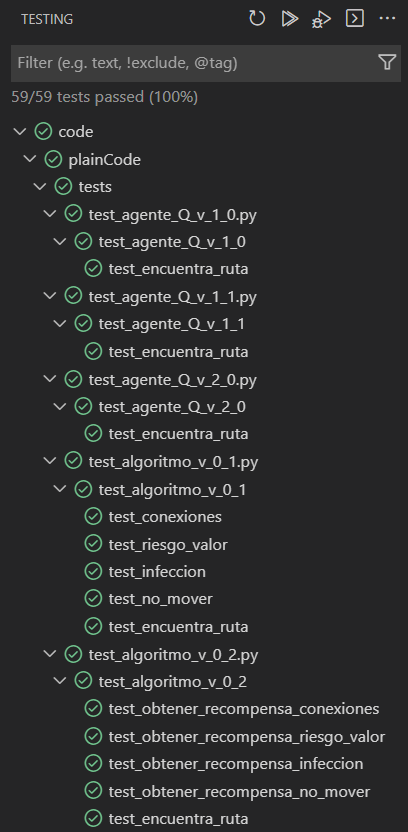
\includegraphics[width=0.6\textwidth]{tests1}
	\caption{Casos de prueba del proyecto. Parte 1}\label{fig:tests1}
\end{figure}
\begin{figure}[!h]
	\centering
	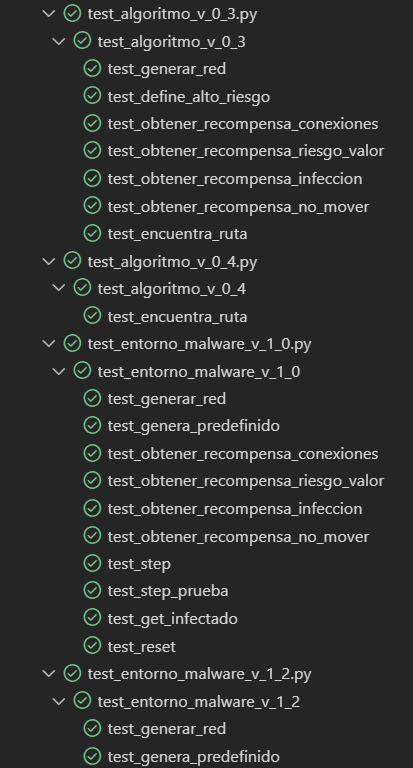
\includegraphics[width=0.6\textwidth]{tests2}
	\caption{Casos de prueba del proyecto. Parte 2}\label{fig:tests2}
\end{figure}
\begin{figure}[!h]
	\centering
	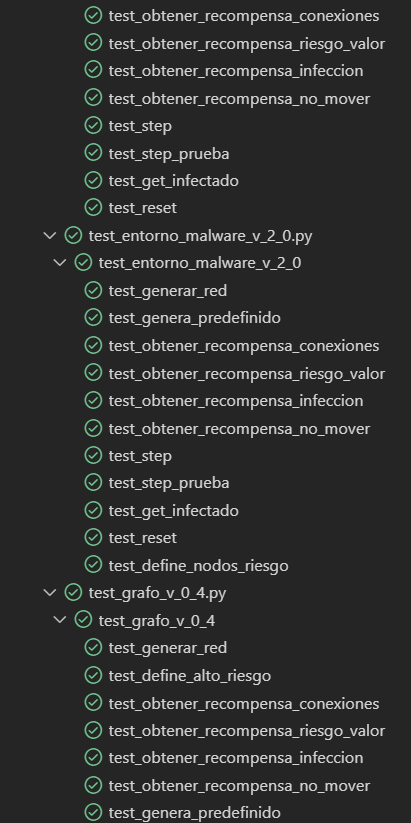
\includegraphics[width=0.6\textwidth]{tests3}
	\caption{Casos de prueba del proyecto. Parte 3}\label{fig:tests3}
\end{figure}
\FloatBarrier

\subsection{Estudio de valores de entrenamiento}
 
 Además de las pruebas unitarias, se decidió realizar un estudio de los valores de entrenamiento, para encontrar qué valores era recomendable asignar a cada variable para obtener resultados de manera consistentemente más rápida.
 
 \subsubsection{Realización del estudio}
 
 Se probó a modificar los siguientes parámetros:
 \begin{itemize}
     \item \textbf{Red de ordenadores:} se utilizaron la tercera, cuarta y quinta redes predefinidas en el código, formadas por 30, 300 y 3000 nodos respectivamente. Se hizo esto para cubrir diferentes situaciones y contextos en los cuales observar la influencia del resto de parámetros en el entrenamiento.
    \item \textbf{Tasa de aprendizaje (variable $\alpha$):} ya que es recomendable un valor entre 0 y 1, pero un valor de 0 resultaría en que no hubiese aprendizaje, se tomaron los valores con cifras decimales impares. Se pudo ver que un valor de 0.1 no aportaba mucha información relevante, así que se simplificó a los valores de 0.3, 0.5, 0.7 y 0,9.
    \item \textbf{Factor de descuento (variable $\gamma$):} también es un valor que debe estar entre 0 y 1, pero en este caso 0 es un número válido, por lo que se tomaron valores con cifras decimales pares, eliminando algunos que se consideraron similares a los demás para evitar una cantidad desorbitada de experimentos. Se acabaron usando los valores 0.2, 0.4, 0.8 y 1.
    \item \textbf{Número de episodios:} debido a los diferentes tamaños de las redes, se necesitaban diferentes números de episodios para realizar entrenamientos satisfactorios. Por ello, se definieron los valores de 5, 50, 100 y 200, pues con 200 se era capaz de entrenar la el entorno más grande de los seleccionados sin problema, y así se cubría un gran rango de valores. Sin embargo, estos números de episodios tan elevados no tenían sentido en redes pequeñas, pues se encontraba la ruta óptima mucho antes, por lo que no ofrecían información estos experimentos, y se decidieron eliminar. 
 \end{itemize}
\newpage

 \begin{table}[h]
\centering
\begin{tabular}{|l|cccc|}
\hline
\textbf{Parámetro}  & \multicolumn{4}{c|}{\textbf{Valores}}    \\ \hline
Nodos de la red     & 30      & \multicolumn{2}{c}{300} & 3000 \\ \hline
Tasa de aprendizaje & 0,3     & 0,5     & 0,7           & 0,9  \\ \hline
Factor de descuento & 0,2     & 0,4     & 0,8           & 1    \\ \hline
Número de episodios & 5       & 50      & 100           & 200  \\ \hline
\end{tabular}
\caption{Valores de los parámetros de los experimentos}
\label{tab:valores-experimentos}
\end{table}


 Se realizó un experimento con cada posible combinación de parámetros. Como se explica en el apartado de Aspectos Relevantes en la memoria principal, estos experimentos consistían en la realización del entrenamiento del agente con dichos parámetros, con la particularidad de que al final de cada episodio se realizaba una búsqueda de la ruta y se registraba su puntuación, pudiendo ver así el progreso del aprendizaje.
 
\imagen{graficaExperimento}{Ejemplo de gráfica obtenida al realizar uno de los experimentos}
 
 Debido a las recompensas definidas para el Proceso de Decisión de Markov del proyecto, cuando el algoritmo no encontraba la ruta obtenía una recompensa negativa de una magnitud considerablemente mayor a la recompensa positiva obtenida al encontrar una ruta óptima. Por lo tanto, en el eje Y las gráficas se obtiene una escala muy grande, que hace difícil visualizar la evolución a partir del momento en el cual se encuentra una ruta hasta el objetivo, pero muestra muy claramente el momento en el que el algoritmo encuentra esa ruta. Este segundo valor es el que se comparó en el estudio.
 
 \subsubsection{Resultados obtenidos}
 Los resultados fueron los siguientes:

\begin{itemize}
    \item En cuanto al \textbf{número de episodios}, con 50 es generalmente suficiente para redes de hasta 300 nodos, pero a partir de esos valores, aunque en general puede seguir ocurriendo que se encuentre la ruta pronto, es cada vez más posible que no se encuentre a tiempo, por lo que se recomienda aumentar el número de episodios, por ejemplo a 100.
    
    \imagen{estudioEpisodios}{Ejemplos del número de episodios que se tarda en converger dependiendo del tamaño de la red}
    
    \item Se descubrió que, generalmente, la \textbf{tasa de aprendizaje} acelera el proceso de entrenamiento a medida que va aumentando. Sin embargo, con redes grandes, valores muy elevados resultaron en que el algoritmo tardase más en encontrar una ruta. Por ello, se decidió recomendar un $\alpha$ de 0,9 en redes de hasta 300 nodos, y valores ligeramente menores a partir de entonces.
    
    \imagen{estudioAlpha}{Ejemplos de la influencia de la tasa de aprendizaje en la velocidad de convergencia}
    
    \item Por otro lado, se observó como la \textbf{tasa de descuento} acabó influyendo con menos frecuencia en los resultados. Sin embargo, se pudo ver como la mayoría de las veces, a valores mayores, el entrenamiento encontraba resultados ligeramente antes que en los otros experimentos, pero cuando se acercaba a valores de 1, volvía a aumentar el tiempo hasta la convergencia. Por lo tanto, se recomendó utilizar un $\gamma$ de 0,8 aunque, como se dice antes, tiene menor influencia sobre los resultados que la tasa de aprendizaje.
    
    \imagen{estudioGamma}{Ejemplos de la influencia del factor de descuento en la velocidad de convergencia}
    
\end{itemize}